\chapter{Knowledge Graphs}
\label{cha:knowledge_graphs}

Knowledge graphs are graph-structured knowledge bases. They store information in the form of relationships between entities. A single information in the graph is referred to as fact. It consist of two entities and a relation between those two. This can be expressed as a triple: $(head, relation, tail)$. Knowledge Graphs are referred to as graphs since their entities can be interpreted as nodes and the relations as labelled and directed edges in a graph. The label here indicates which kind of relation the entities share and the direction indicates which entity is the head entity and which the tail entity i.e. an edge points from the head to the tail. An example for a knowledge graph can be seen in figure \ref{fig:example_kg}. \cite{nickel_review_2015}

\begin{figure}[H]
\centering
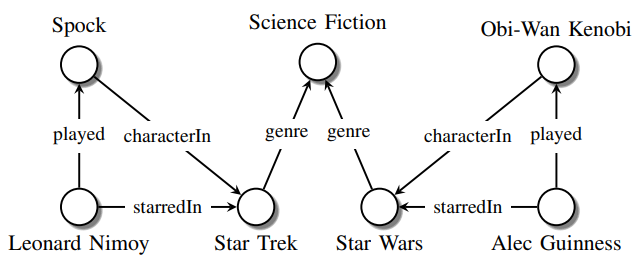
\includegraphics[width=0.9\textwidth]{images/example_kg.png}
\caption{Example of a Knowledge Graph}
\label{fig:example_kg}
\end{figure}

The term 'knowledge graph' was first introduced by Google in 2012 \cite{singhal_introducing_2012}. In their blog they spoke about how they use their knowledge graph to enrich search engine results. The most noticeable part of how they use knowledge graphs are the side windows when searching for an entity with their search engine. An example of such can be seen in figure \ref{fig:side_window_google}. Here we can see what kind of knowledge Google has about the University of Mannheim. For example it seems to be that \textit{(University of Mannheim, founded\_in, 1907)} is one of the facts in their Knowledge Graph.

\begin{figure}[H]
\centering
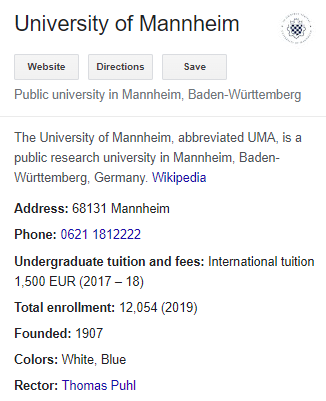
\includegraphics[width=0.5\textwidth]{images/example_google_side_window.png}
\caption{Example of a Google Side Window}
\label{fig:side_window_google}
\end{figure}

In the recent years knowledge graphs have become more and more popular and have found their way into further applications than search engines. An overview of applications can be seen in figure \ref{fig:application_kg}.   Question Answering systems use knowledge graphs to enhance their results. Examples here include social chatbots and digital assistance like Siri. Recommender Systems leverage knowledge graphs as side information to improve and diversify their recommendations.  Moreover, knowledge graphs are also used in information retrieval, domain-specific applications and more. \cite{zou_survey_2020}

\begin{figure}[H]
\centering
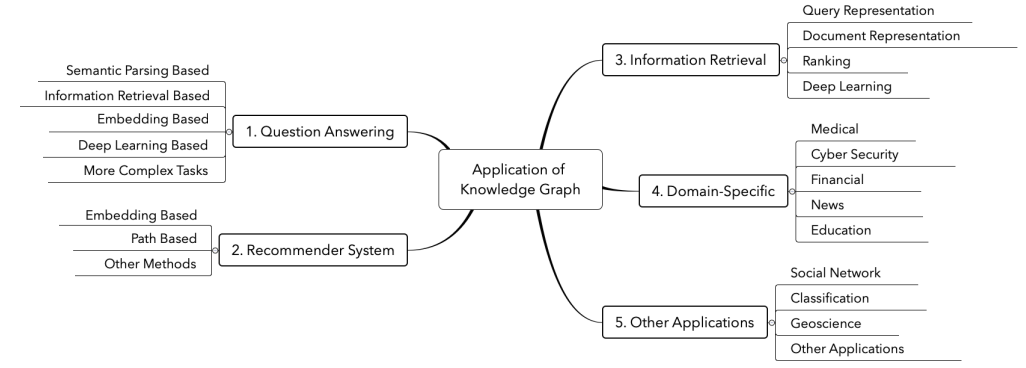
\includegraphics[width=0.9\textwidth]{images/applications_kg.png}
\caption{Applications of Knowledge Graphs}
\label{fig:application_kg}
\end{figure}

According to Paulheim \cite{paulheim_knowledge_2016} a knowledge graph is defined by the following four characteristics: 

\begin{enumerate}
\item "mainly describes real world entities and their interrelations, organized in a graph"
\item "defines possible classes and relations of entities
in a schema"
\item "allows for potentially interrelating arbitrary entities with each other"
\item "covers various topical domains"
\end{enumerate}

The first characteristic defines that knowledge graphs consist of two kind of instances, entities and relations. An entity can be almost everything from an individual person to any kind of object. These entities are then linked through different kind of relations, which forms our graph. 

The schema of the graph plays only a minor role. In most cases the instance-level statements (entities and triples) far outnumber the schema-level statements (entity classes and relations). 

With the third characteristic Paulheim opens up the possibility that there are arbitrary relations between entities which are not included in the knowledge graph. The chapter \ref{cha:knowledge_graph_completion} will discuss this further. 

Lastly, another characteristic of knowledge graphs is that they do not focus on a single domain but interlink multiple topical domains. 